\documentclass[12pt]{article}
\usepackage[a4paper, margin=.30in]{geometry}
\usepackage{graphicx ,
            wrapfig,
            xcolor, 
            enumerate,
            amsmath,fontenc,
            tcolorbox,mathrsfs
            }
\usepackage{mathptmx}
\usepackage[siunitx, RPvoltages]{circuitikz}
\newcommand\headerMe[2]{\noindent{}#1\hfill#2}
\renewcommand{\thesection}{\Roman{section}}

\author{Zakaria HAOUZAN}
\date{\today}

\begin{document}
% headers --------------
\headerMe{Matière : Physique-Chimie}{Professeur : Zakaria HAOUZAN}\\
\headerMe{Unité : Electricité}{Établissement : Lycée SKHOR qualifiant}\\
\headerMe{Niveau : 1BAC-SM/X}{Heure : 17H/12H}\\

% ------Content ________

%\begin{wrapfigure}[10]{r}{0.5\textwidth}
    %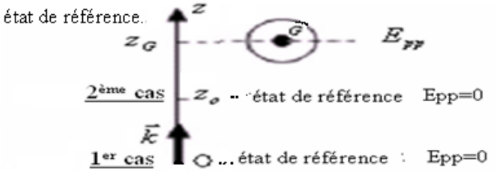
\includegraphics[width=0.5\textwidth]{./img/img00.png}
%\end{wrapfigure}


%\begin{tcolorbox}[colback=black!15!white,
                  %colframe=black!10!black,
                  %title=Remarque :
                 %]
\begin{center}

    \Large{Leçon $N^{\circ} 8 $: \color{red}Champ magnétique créé par un courant électrique }
\end{center}

\begin{wrapfigure}[5]{r}{0.3\textwidth}
  \vspace{-3cm}
    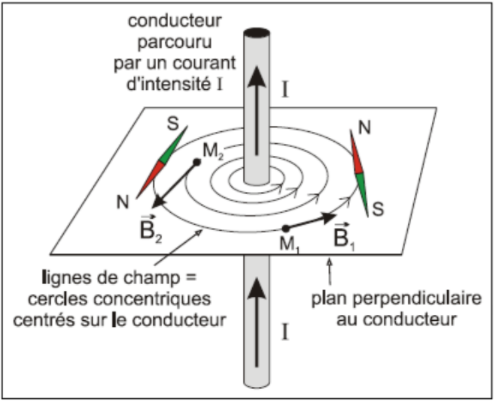
\includegraphics[width=0.3\textwidth]{./img/Un fil de longueur.png}
\end{wrapfigure}
  \section{ Champ magnétique créé un fil rectiligne:}
  \subsection{spectre du champ magnétique :}
Un fil de longueur infinie parcouru par un courant
d’intensité I, crée un champ magnétique dont les
lignes de champ sont des cercles concentriques
centrés sur le fil et situé dans le plan perpendiculaire
au fil.
  Remarque :\\ si le vecteur champ magnétique est perpendiculaire au plan et dirigé vers l'avant on le représente par :$\vec{B}$ .
  \\ si le vecteur champ magnétique est perpendiculaire au plan et dirigé vers l'arrière on le représente par :$\vec{B}$ +
\begin{wrapfigure}[]{r}{0.2\textwidth}
  \vspace{-1cm}
    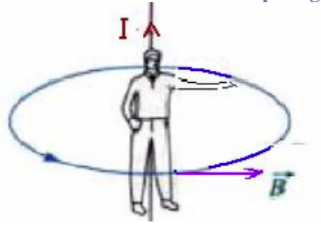
\includegraphics[width=0.2\textwidth]{./img/l'observateur.png}
    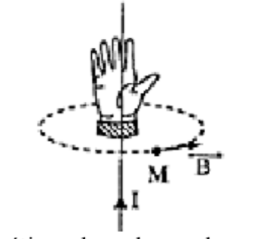
\includegraphics[width=0.2\textwidth]{./img/main droite.png}
\end{wrapfigure}
  \subsection{Caractéristiques du vecteur champ
magnétique :}

  Direction : portée par la tangente au cercle du spectre passant par M.

  Intensité : donnée par la relation : $$B = \frac{\mu_0}{2\pi}.\frac{I}{d}$$ 
  \\B : intensité du champ magnétique au point M en (T).
\\$\mu_0$: perméabilité magnétique du vide (ou de l’aire) sa valeur est $\mu_0 = 4\pi.10^-7$ (S.I)
\\I : intensité du courant.
\\d = OM : La distance du point M au fil en (m) .
 
  donc $B = 2.10^-7.\frac{I}{d}$

  Sens : donné par les règles d’orientation.

  \begin{enumerate}
    \item[a] Règle de l'observateur d'Ampère : L'observateur couché le long du fil de façon que le courant électrique circule de ses pieds vers sa tète, et regardant au point M, sa main gauche tendue indique la direction et le sens du vecteur champ magnétique au point M

    \item[b] Règle de la main droite : En plaçant la main droite le long du fil de façon que les doigts soient dirigés dans le sens du courant électrique, la
paume de la main orientée vers le point M, le pouce tendu indique le sens du vecteur champ magnétique au point M.

  \end{enumerate}

  Exemples : représenter le vecteur champ magnétique dans chacun des cas suivants:

    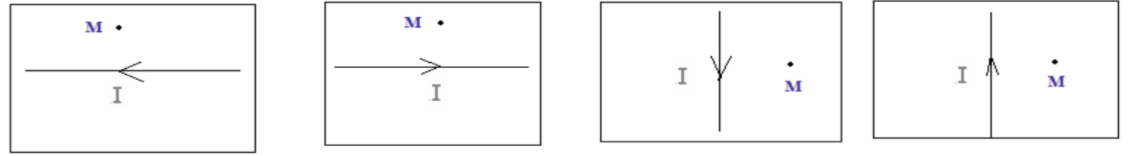
\includegraphics[width=1\textwidth]{./img/Exemple.png}

\begin{wrapfigure}[2]{r}{0.4\textwidth}
  %\vspace{-1cm}
    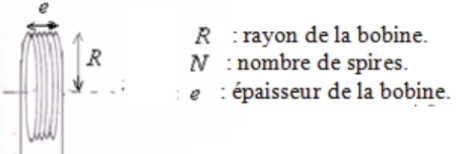
\includegraphics[width=0.4\textwidth]{./img/bobine plate.png}

\end{wrapfigure}

  \section{Champ magnétique créé par une bobine plate :}
La bobine plate un circuit électrique circulaire formé par plusieurs spires conductrices et dont le rayon est très
grand devant son épaisseur.

\begin{wrapfigure}[]{r}{0.3\textwidth}
  %\vspace{-1cm}
    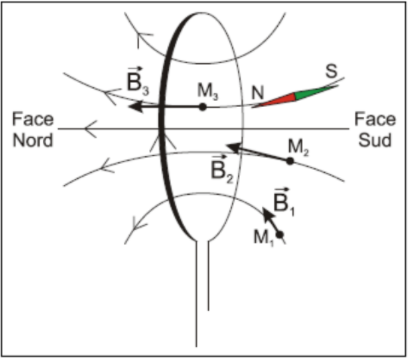
\includegraphics[width=0.3\textwidth]{./img/SpectreBobine_plate.png}
    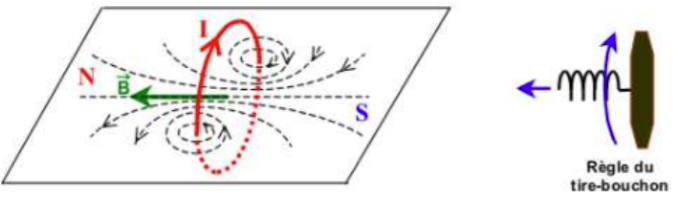
\includegraphics[width=0.3\textwidth]{./img/spect_2plate.png}

\end{wrapfigure}
\subsection{ Spectre du champ magnétique}
Dans un plan perpendiculaire au plan de la bobine et
contenant son centre, les lignes de champ sont des droites
rectilignes près du centre et s’incurvent en s’éloignant de
celui-ci pour devenir des cercles fermés près des fils
conducteurs.

\subsection{sens du vecteur champ magnétique :}

Le sens du vecteur champ magnétique est déterminé par la règle du bonhomme d’Ampère ou de la
main droite.

La face nord de la bobine est la face par laquelle sortent les lignes de champ.

La face sud de la bobine est la face par laquelle entrent les lignes de champ.

On regarde l’une des faces :

- s’il correspond au sens indiqué par la lettre S on regarde sur la face sud.

- s’il correspond à celui indiqué par la lettre N on regarde sur la face nord.

\begin{center}
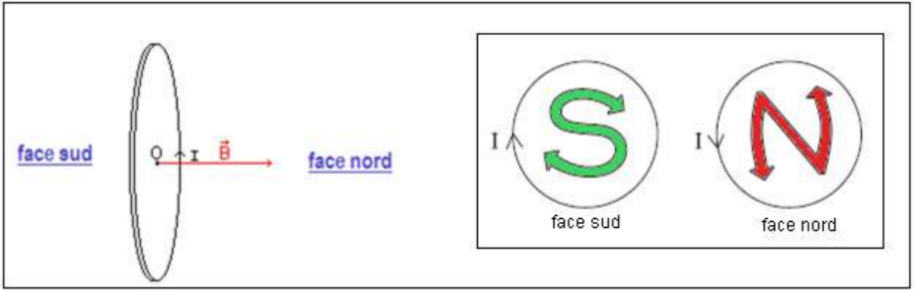
\includegraphics[width=1\textwidth]{./img/sens_plate_mag.png}
\end{center}


\subsection{Intensité :}
L’intensité du champ magnétique crée par une bobine plate de rayon R, contenant N spires et
parcouru par un courant continu I en son centre O est :
$$B = \frac{\mu_0}{2}.\frac{N.I}{R}$$
Avec : $\mu_0 = 4\pi.10^{-7}(S. I)$

\section{Champ magnétique créé par un solénoïde :}

Un solénoïde est constitué d’un fil conducteur enroulé sur un cylindre
isolant dont la longueur est très grande.

\subsection{spectre du champ magnétique : }
A l’intérieur d’un solénoïde les lignes de champ sont des droites parallèles,
le champ est donc le champ est uniforme.
\begin{center}
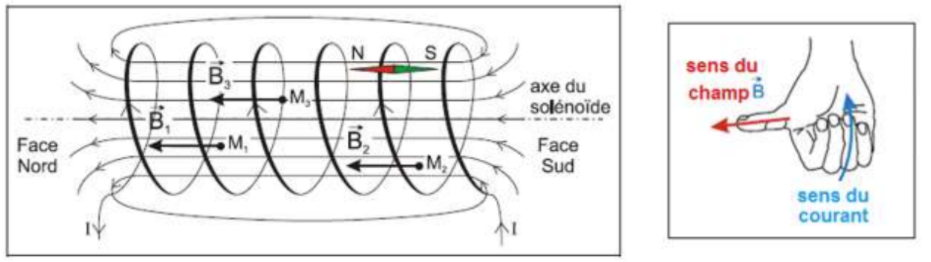
\includegraphics[width=1\textwidth]{./img/solénoïde_Spectre.png}
\end{center}
A l’extérieur du solénoïde, le spectre magnétique ressemble à celui d’un aiment droit.

\subsection{sens du vecteur champ magnétique :}
Règle de la main droite (valable dans tous les cas) :
\\Pouce : sens de $\vec{B}$
\\Doigts courbés : sens du courant I
\begin{center}
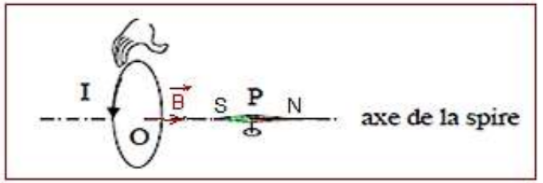
\includegraphics[width=0.6\textwidth]{./img/solen_sens.png}
\end{center}

\subsection{Intensité du champ magnétique :}

A l’intérieur du solénoïde le champ magnétique est uniforme d’intensité
$$B = \mu_0.\frac{N}{L} = \mu_0.n.I$$

Avec : $\mu_0 = 4\pi.10^{-7}(S. I)$

n : densité de spires : n =N/L
avec L : longueur du solénoïde et N : nombre de spires.

I : intensité du courant à travers le solénoïde. Le sens de $\vec{B}$ dépend du sens de I.

\end{document}

